\documentclass[conference]{IEEEtran}
\usepackage{cite}
\usepackage{amsmath,amssymb,amsfonts}
\usepackage{algorithm}
\usepackage[noend]{algpseudocode}
\usepackage{graphicx}
\usepackage{varwidth}
\usepackage{textcomp}
\usepackage{xcolor}
\usepackage[printonlyused,withpage]{acronym}

\acrodefplural{GA}[GA's]{genetic algorithms}

\makeatletter
\def\BState{\State\hskip-\ALG@thistlm}
\makeatother

\def\BibTeX{{
	\rm B\kern-.05em{\sc i\kern-.025em b}\kern-.08em
	T\kern-.1667em\lower.7ex\hbox{E}\kern-.125emX
}}

\begin{document}
	
	\title{Genetic Algorithm Development Platform}
	
	\author{\IEEEauthorblockN{R. Nicholas Vandemark}
		\IEEEauthorblockA{\textit{University of Maryland} \\
			\textit{ENPM690 - Robot Learning, Project}\\
			nickvand@umd.edu}
	}
	
	\maketitle
	
	\begin{abstract}
		Research on generalization of genetic algorithms pertaining to robot learning is discussed. Algorithms utilizing these generalizations were designed, and a platform implementing these algorithms was developed to autonomously train the agents (agnostic to robot structure and its objective) in simulation via a simulation suite.
	\end{abstract}
	
	\begin{IEEEkeywords}
		Genetic algorithms, robot learning, Gazebo, ROS2 control
	\end{IEEEkeywords}
	
	\section{Introduction}

	A \ac{GA} is an optimization technique that is inspired by Darwinian evolution. Iterations of the algorithm test the performance of each ``chromosome'' (a possible solution to the function which is to be optimized) in the ``population'' (a list of these solutions), which is initially randomly generated. After evaluating the performance of each chromosome, some which had the best performances ``reproduce'' to create new chromosomes, which replace those which had the worst performances in the population. This emulates survival of the fittest in nature. Each time the population goes through this reproduction cycle, these chromosomes are given a chance to mutate by some small amount because these slight differences could produce even better performance, which emulates random biological mutation that persists. This procedure converges when a chromosome performs well enough (according to desired training criteria).

	The objective for this project was to create a platform that can be used to simultaneously develop/tune robot controllers that learn their behaviors from \acp{GA} via simulation and then seamlessly use this tuned controller on any medium (simulated, hardware, etc.). Furthermore, the core of this platform should be able to be used for many different types of robots and objectives (i.e., it should be agnostic to the structure of a robot and the behavior it is learning), so that it can be used for more than one specific scenario. The core functionality should have an emphasis on generalizing the pipeline for training this type of controller, such that training new agents and/or behaviors is as lightweight in development as possible, but that the platform remains \textit{entirely} agnostic to the structure and interfaces of robotic agents. Examples would be motion controllers for serial, parallel, or differential drive robots with any types of completion criteria.

	\section{Methodology}

	\subsection{Technologies}

	This platform is implemented on top of the \textit{ROS2} software stack, and the chosen simulation suite was Gazebo. These choices were made with many considerations in mind.

	The \textit{ros2\textunderscore control} packages \cite{ros2-control} offer interfaces to robot control theory on top of the \textit{ROS2} software stack, with a strong emphasis on agnosticism to the system that the controllers are being developed towards in an effort to support as many configurations as possible. Similar to how connections between publishers and subscribers in a ROS2 network are ``named", the interfaces of the controllers owned by a \textit{ROS2 control}'s \textit{controller manager} node are also named. This allows for dynamically configurable connections between the robot's hardware and its controller(s), but unlike traditional publishers/subscribers, these connections only communicate decimal values, whose values make sense with the context of the control problem (these could be joint positions, joint velocities, battery charge percentages, etc.). Along with the tools in these packages are implementations of commonly used controllers and hardware interfaces. \textit{ros2\textunderscore control} was therefore chosen for its significant support for dynamic configurability and agnosticism to types of control, which is important in a system which aims to be as agnostic to the robot's structure/hardware as possible.

	Gazebo was chosen for its compatibility with \textit{ROS2}, but also primarily because of a plugin offered by the \textit{gazebo\textunderscore ros2\textunderscore control} package \cite{gazebo-ros2-control} which allows for the utilities in the \textit{ros2\textunderscore control} packages to easily interface with the functionality of Gazebo. This plugin allows the developer to easily bind the telemetry of the simulated robotic agent to the state interfaces managed by a \textit{controller manager} node, and also bears the burden of the controller manager node's lifecycle. Because Gazebo can be configured to use many different types of physics engines with different configuration parameters, this means that the controller's \ac{GA} is being trained on as accurate a simulation as desired.

	\subsection{Design}

	The implementation of this platform consists of four main packages \cite{git-repo} (where the \textit{ep} prefix simply stands for ``ENPM690 project''):
	\begin{itemize}
		\item \textit{ep\textunderscore common}: This contains node interfaces / utilities used in both runtime and training configurations. Most notably, this includes the command interface controller interface, which is responsible for directly forwarding the outputs of a genetic algorithm's fitness function to the command interfaces requested in the training campaign.
		\item \textit{ep\textunderscore common\textunderscore interfaces}: This contains basic ROS2 messages, services, etc used in both runtime and training configurations.
		\item \textit{ep\textunderscore training}: This contains node interfaces / utilities used only in training configurations. This includes many of the nodes used in the training configuration, such as the genetic algorithm controller interface (the master node of this configuration), the state observer interface, the fitness evaluator interface and an extension of it which depends on time (it subscribes to the clock of the simulation for ease of use), and the campaign orchestrator GUI.
		\item \textit{ep\textunderscore training\textunderscore interfaces}: This contains ROS2 messages, services, etc used only in training configurations. This includes the custom action for executing training campaigns.
	\end{itemize}

	Figures~\ref{fig:runtime_configuration} and~\ref{fig:training_configuration} show the \textit{ROS2} nodes needed for the runtime and training configurations of the system, respectively. Each node label that has the suffix ``1..N'' could theoretically have multiple instances, so the training campaign could be parallelized. The topics used by these nodes are also indexed according to the ``i'' suffix of those names.

	Figure~\ref{fig:runtime_configuration} shows that the runtime configuration uses a Gazebo instance, but this could also be a hardware robot, some other simulated version of it, etc. The only other node is the robot controller, which uses the fitness function of the \ac{GA} with the requested configuration parameters (learned through previous training) to control the behavior of the robot.
	
	\begin{figure}[htbp]
		\centerline{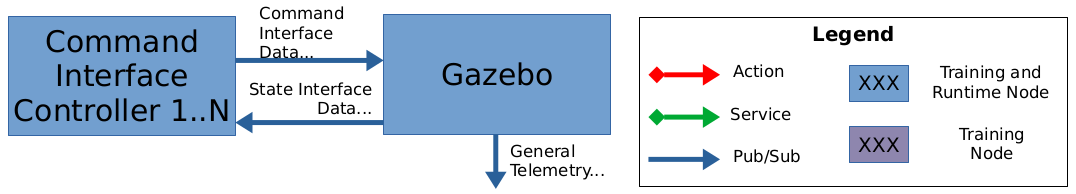
\includegraphics[width=\columnwidth]{images/runtime_configuration.png}}
		\caption{The configuration of the system on runtime.}
		\label{fig:runtime_configuration}
	\end{figure}

	\begin{figure}[htbp]
		\centerline{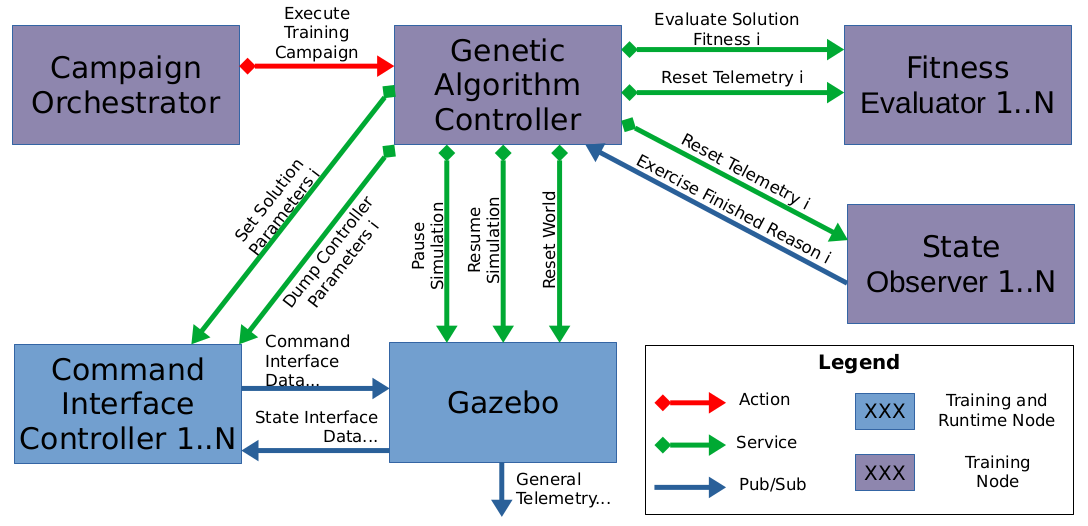
\includegraphics[width=\columnwidth]{images/training_configuration.png}}
		\caption{The configuration of the system while training.}
		\label{fig:training_configuration}
	\end{figure}

	It can be seen that the architecture of Figure~\ref{fig:training_configuration} is a superset of that in Figure~\ref{fig:runtime_configuration}, and this is because each iteration of the genetic algorithm controller node's main routine essentially runs a short-lived instance of the runtime configuration with different configuration parameters while other nodes observe its behavior during the simulation. These additional nodes can be described as the following:
	\begin{itemize}
		\item \textit{Genetic Algorithm Controller}: This is essentially the master node of the training configuration. It implements the generalized genetic algorithm, including creating the initial randomly-generated population, the crossover routine, and the mutation routine. Again, this is agnostic to the structure of the robot and the behavior being trained, up until the exact datatype of the solution. As the training campaign runs, this node will take a chromosome out of the population, convert it to ROS2 parameters, set the configuration of the robot controller with these parameters, simulate its performance by manipulating the state of the simulation, and collect its quantified performance. This overall procedure is described in Algorithm~\ref{alg:ga-controller-training-routine}, and the higher-level procedures referenced therein are broken out into Algorithms~\ref{alg:ga-controller-secondary-routines} to~\ref{alg:ga-controller-ros2-service-calls}. The procedures in Algorithm~\ref{alg:ga-controller-specific-routines} are implemented specific to the structure of a chromosome. While they must be implemented for each new datatype, they can be used to train any number of behaviors for a system that utilizes this datatype.
		\item \textit{State Observer}: Once simulation starts, this node is responsible for detecting when an individual solution's completion criteria has been met by listening to the robot's telemetry. Once met, it informs the genetic algorithm controller which criteria was met. By default, this node will observe when the timeout has been met/exceeded, but observing other criteria is implemented for each desired behavior.
		\item \textit{Fitness Evaluator}: This node performs any desired metrics on telemetry output by the robot over the course of the simulation to quantify the performance of a solution. This result is used by the genetic algorithm controller to compare the performances of the chromosomes in a population. Notably, this node does not have an implementation of the fitness function (only the robot controller does). This implies that the quantifiable performance of a chromosome is not the direct output of the fitness function, but how it manifests behavior in the simulated environment.
		\item \textit{Campaign Orchestrator}: This node provides a user interface for executing training campaigns via the genetic algorithm controller. It provides user inputs for each of the hyperparameters in a custom ROS2 action (many of the inputs to the \textit{ExecuteTrainingCampaign} procedure of Algorithm~\ref{alg:ga-controller-training-routine}), and displays (read-only) feedback as the campaign proceeds. A screenshot of this user interface can be seen in Figure~\ref{fig:campaign_orchestrator_ui}.
	\end{itemize}

	\begin{algorithm}
		\caption{Genetic algorithm controller training routine}
		\label{alg:ga-controller-training-routine}
		\begin{algorithmic}[1]
			\Procedure{ExecuteTrainingCampaign}{gen\textunderscore count, gen\textunderscore soln\textunderscore count, soln\textunderscore time\textunderscore limit, conv\textunderscore th, num\textunderscore offspring, mutability, cmnd\textunderscore if, state\textunderscore if}
			\State $\textit{gen\textunderscore number} \gets 0$
			\State $\textit{pop} \gets Null$ \Comment{The population of solutions}
			\State $\textit{PauseSimulation()}$
			\Loop
			\If {$\textit{gen\textunderscore number}$ = 0}
			\State $\textit{pop} \gets \textit{InitPopulation(gen\textunderscore soln\textunderscore count)}$
			\Else
			\State $\textit{pop} \gets \textit{Select(pop)}$
			\State $\textit{pop} \gets \textit{Crossover(pop, num\textunderscore offspring)}$
			\State $\textit{pop} \gets \textit{Mutate(pop, mutability)}$
			\EndIf
			\ForAll{$\textit{soln}$ in $\textit{pop}$}
			\State $\textit{params} \gets \textit{GetParams(soln, cmnd\textunderscore if, state\textunderscore if)}$
			\State $\textit{SetControllerParams(params)}$
			\State $\textit{ResetSimulation()}$
			\State $\textit{RestartStateObserver(soln\textunderscore time\textunderscore limit)}$
			\State $\textit{RestartFitnessEvaluator()}$
			\State $\textit{PlaySimulation()}$
			\State $\textit{WaitForSimulatedSolnCompletionCriteria()}$
			\State $\textit{PauseSimulation()}$
			\State $\textit{soln\textunderscore fitness} \gets \textit{EvaluateSolnPerformance()}$
			\If {$\textit{CompareFitness(soln\textunderscore fitness, conv\textunderscore th)}$}
			\State \Return $\textit{gen\textunderscore number, soln, soln\textunderscore fitness}$
			\EndIf
			\EndFor
			\State increment $\textit{gen\textunderscore number}$
			\If {$\textit{gen\textunderscore number}$ = $\textit{gen\textunderscore count}$}
			\State \Return $Null$
			\EndIf
			\EndLoop
			\EndProcedure
		\end{algorithmic}
	\end{algorithm}

	\begin{algorithm}
		\caption{Genetic algorithm controller secondary routines}
		\label{alg:ga-controller-secondary-routines}
		\begin{algorithmic}[1]
			\Procedure{InitPopulation}{gen\textunderscore soln\textunderscore count}
			\State $\textit{pop} \gets$ Empty List
			\For{$\textit{i}$ = 0 to $\textit{gen\textunderscore soln\textunderscore count}$}
			\State $\textit{rand\textunderscore soln} \gets \textit{GetRandomSoln()}$
			\State append $\textit{rand\textunderscore soln}$ to $\textit{pop}$
			\EndFor
			\State \Return $\textit{pop}$
			\EndProcedure

			\Procedure{Select}{pop}
			\State $\textit{pop\textunderscore sorted} \gets pop$ sorted via $\textit{CompareFitness}$
			\State \Return $\textit{pop\textunderscore sorted}$
			\EndProcedure
			
			\Procedure{Crossover}{pop, num\textunderscore offspring}
			\State $\textit{num\textunderscore solns} \gets size(pop)$
			\For{$\textit{i}$ = 0 to $\textit{num\textunderscore offspring}$}
			\State $\textit{parent0} \gets i$
			\State $\textit{parent1} \gets i+1$
			\State $\textit{offs0} \gets \textit{num\textunderscore solns - parent0}$
			\State $\textit{offs1} \gets \textit{num\textunderscore solns - parent1}$
			\State $\textit{rand\textunderscore crossover\textunderscore point} \gets \textit{Random(0.0, 1.0)}$
			\State \begin{varwidth}[t]{\linewidth}
				$\textit{pop[offs0], pop[offs1]} \gets \textit{DoCrossoverAt(}$\par
					\hskip\algorithmicindent $\textit{pop[parent0],}$\par
					\hskip\algorithmicindent $\textit{pop[parent1],}$\par
					\hskip\algorithmicindent $\textit{rand\textunderscore crossover\textunderscore point})$
			\end{varwidth}
			\EndFor
			\State \Return $\textit{pop}$
			\EndProcedure
			
			\Procedure{Mutate}{pop, mutability}
			\For{$\textit{i}$ = 0 to $\textit{size(pop)}$}
			\State $\textit{pop[i]} \gets \textit{MutateSoln(pop[i], mutability)}$
			\EndFor
			\State \Return $\textit{pop}$
			\EndProcedure
			
			\Procedure{WaitForSimulatedSolnCompletionCriteria}{}
			\State $\textit{finished\textunderscore reason} \gets$ NOT\textunderscore FINISHED
			\While{$\textit{finished\textunderscore reason}$ = NOT\textunderscore FINISHED}
			\State $\textit{msg} \gets SolnCompletionCriteriaCallback()$
			\State $\textit{finished\textunderscore reason} \gets \textit{msg.value}$
			\EndWhile
			\EndProcedure
		\end{algorithmic}
	\end{algorithm}

	\begin{algorithm}
		\caption{Genetic algorithm controller routines that are specific to solution type}
		\label{alg:ga-controller-specific-routines}
		\begin{algorithmic}[1]
			\Procedure{GetRandomSoln}{}
			\Comment{Returns a randomly generated solution.}
			\EndProcedure
			\Procedure{CompareFitness}{f0, f1}
			\Comment{Returns true if f0 is a better fitness than f1, false otherwise.}
			\EndProcedure
			\Procedure{DoCrossoverAt}{soln0, soln1, crossover}
			\Comment{Returns the two offspring of the two given chromosomes at the given crossover [0.0,1.0].}
			\EndProcedure
			\Procedure{MutateSolution}{soln, mutability}
			\Comment{Returns the given solution randomly mutated within the boundaries of the given mutability.}
			\EndProcedure
			\Procedure{GetParams}{soln, cmnd\textunderscore if, state\textunderscore if}
			\Comment{Returns the set of parameters to fully define the robot control parameters, consisting of at least the given robot command and state interface names.}
			\EndProcedure
		\end{algorithmic}
	\end{algorithm}

	\begin{algorithm}
		\caption{Genetic algorithm controller ROS2 subscription callbacks}
		\label{alg:ga-controller-ros2-subscription-callbacks}
		\begin{algorithmic}[1]
			\Procedure{SolnCompletionCriteriaCallback}{}
			\Comment{ep\textunderscore training\textunderscore interfaces/ExercisingSolutionFinishedReason}
			\EndProcedure
		\end{algorithmic}
	\end{algorithm}

	\begin{algorithm}
		\caption{Genetic algorithm controller ROS2 service calls}
		\label{alg:ga-controller-ros2-service-calls}
		\begin{algorithmic}[1]
			\Procedure{PauseSimulation}{}
			\Comment{std\textunderscore srvs/Empty}
			\EndProcedure
			\Procedure{ResetSimulation}{}
			\Comment{std\textunderscore srvs/Empty}
			\EndProcedure
			\Procedure{PlaySimulation}{}
			\Comment{std\textunderscore srvs/Empty}
			\EndProcedure
			\Procedure{SetControllerParams}{}
			\Comment{rcl\textunderscore interfaces/SetParameters}
			\EndProcedure
			\Procedure{RestartStateObserver}{}
			\Comment{ep\textunderscore common\textunderscore interfaces/SetDouble}
			\EndProcedure
			\Procedure{RestartFitnessEvaluator}{}
			\Comment{std\textunderscore srvs/Empty}
			\EndProcedure
			\Procedure{EvaluateSolnPerformance}{}
			\Comment{ep\textunderscore common\textunderscore interfaces/GetDouble}
			\EndProcedure
		\end{algorithmic}
	\end{algorithm}

	\begin{figure}[htbp]
		\centerline{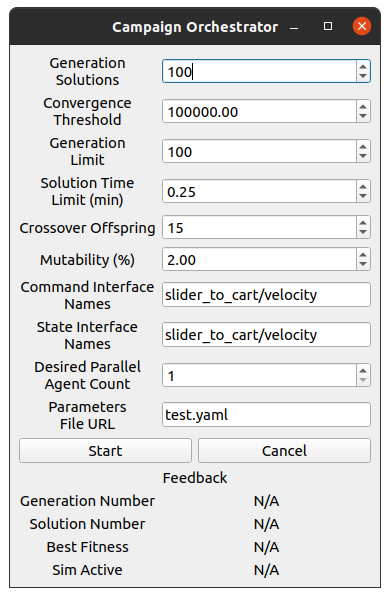
\includegraphics[width=0.75\columnwidth]{images/campaign_orchestrator_ui.png}}
		\caption{An example of the user interface used to request training campaigns with the platform.}
		\label{fig:campaign_orchestrator_ui}
	\end{figure}

	\section{Results}

	Development for the platform made significant progress, but there are a number of technical issues that prevented completion of the platform in the limited timeframe. The way that this platform attempts to use the \textit{ros2\textunderscore control} and \textit{gazebo\textunderscore ros2\textunderscore control} packages seems to be a use case that was not originally supported by them, so extra work will have to go into updating those third-party packages to cope with what this application is intending for.

	\subsection{Current Design}

	The base design for all of the types of nodes seen in Figure~\ref{fig:training_configuration} were completed, with their implementations in the \textit{ep\textunderscore common} and \textit{ep\textunderscore training} packages.

	An example package \textit{ep\textunderscore gantry\textunderscore velocity\textunderscore control\textunderscore demo} was being developed, which is a scenario which uses this platform to train the $K_p$, $K_i$, and $K_d$ parameters of a one degree of freedom gantry's PID velocity controller. Nodes which implement the \textit{robot / command interface controller}, \textit{state observer}, and \textit{fitness evaluator} interfaces were created for this robotic agent and the desired behavior (maintain a given trapezoidal velocity profile). A launch file was created to properly instantiate all of the controllers and nodes, start Gazebo, and set the node parameters.

	However, as mentioned above, there were technical issues which prevented the completion of the core platform, and therefore this example which demonstrates its use as well. The README.md file \cite{git-repo} on this repository's development branch describes how the system can be started, but will fail to proceed.

	\subsection{Future Development}

	There is a critical issue implementing the core of this platform's design, which after initial investigation seems to have to do with how the \textit{ROS2} controller manager node and the node which wraps around Gazebo are executed. Manipulating the state of the physics simulation (pausing, resuming, and resetting) are tricky, but resetting the world and/or simulation somehow disconnects the controllers from the simulated telemetry. Furthermore, this setup does not allow for the controllers under the \textit{controller manager} node to handle callbacks to subscriptions, service calls, etc. while the simulation is paused. The executor does not update if the simulation is paused, which is just fine for the Gazebo node wrapper, but this also prevents the \textit{controller manager} node from updating. This means that while the simulation is paused, the parameters for the robot controller that are a function of the \ac{GA} cannot be updated. This makes continuous simulation of different solutions/chromosomes impossible at the moment, until this is resolved. Doing so is top priority for future development.

	Less critical but still important is the ability to parallelize solutions while in the training configuration, as this would speed up training by a factor directly proportional to the number of parallel agents. This would require support in the genetic algorithm controller and, if the collision bitmask offered in previous versions of Gazebo is still supported, automated generation of this stanza in the robots' URDFs. A nice-to-have would be a visual cue as to which is which, such as color-coding of the entire model.

	\section{Discussion}

	The work-in-progress platform is a professionally developed set of packages with a strong potential to accomplish its goal. Once finished, it could be a powerful tool to assist with semi-automated robot learning for any agent that has support for \textit{ROS2 control} and Gazebo and whose behavior can be reinforced with the hyperparameters offered by the campaign orchestrator's user interface.

	This provides a solid foundation for generalizing the behavior of \acp{GA}, but perhaps this could be built upon more to further generalize the behavior of the larger class of evolutionary algorithms, and the genetic algorithm controller can be broken out into different tiers to cater to different types of evolutionary algorithms. Much of the core behavior that was difficult to organize and implement (coordinating simulation state, packaging and communicating chromosome and robot interface data as ROS2 parameters, standardizing passive telemetry observation, etc.) would remain the same, it would only be the structure around the \textit{InitPopulation}, \textit{Select}, \textit{Crossover}, and \textit{Mutate} routines in Algorithm~\ref{alg:ga-controller-training-routine} that would have to be updated to be more flexible. Not only would this be a useful addition to the platform, but learning how to generalize routines and finding commonality between different ones is a powerful learning tool.

	The aforementioned technical issues that are a function of the chosen technologies could be further explored, and perhaps those technologies could be removed. For example, perhaps the plugin offered by the \textit{gazebo\textunderscore ros2\textunderscore control} could be removed in favor of manually setting up instances of the \textit{controller manager} node and configuring the connections to use the telemetry coming out of the Gazebo simulation. This could have the side-effect of easier transition from simulated and physical robotic agents, as this package would have more control over the \textit{ROS2} connections that for now are left to this third-party plugin.

	\section{Conclusion}

	Considerations were made on how to generalize the concepts of a \ac{GA}, and then algorithms that are to a degree agnostic to the structure of the robotic agent and the behavior being learned were designed. A platform which implements these in a training configuration was designed on top of \textit{ROS2} and with \textit{Gazebo}, and this same platform could also be used to operate the robot controller with the learned behavior in a runtime configuration. A user interface was developed to execute these training campaigns.

	There was significant progress on development for this platform, and a working solution would be ready with some more development to cope with technical issues. Learning not only how to develop genetic algorithms but generalizing their structure with wider applicability was extremely beneficial.

	\section{Acknowledgments}

	This project was done individually, so all contributions belong to R. Nicholas Vandemark.

	\section{List of Acronyms}

	\begin{acronym}
		\acro{GA}{genetic algorithm}
	\end{acronym}
	
	\begin{thebibliography}{00}
		\bibitem{git-repo} R. Nicholas Vandemark,\\
		https://github.com/rnvandemark/enpm690\textunderscore project, 2023.
		\bibitem{ros2-control} ros2\textunderscore control Maintainers,\\
		https://github.com/ros-controls/ros2\textunderscore control/tree/galactic, 2023.
		\bibitem{gazebo-ros2-control} gazebo\textunderscore ros2\textunderscore control Maintainers,\\
		https://github.com/ros-controls/gazebo\textunderscore ros2\textunderscore control/tree/galactic, 2023.
	\end{thebibliography}
	
\end{document}
